\documentclass[cal1spr16Lectures.tex]{subfiles}
%\AtBeginSubsection{
%	\begin{frame}[allowframebreaks]{}
%	\begin{multicols}{2}
%	\tableofcontents[currentsubsection]
%	\end{multicols}
%	\end{frame}
%	}
	
\begin{document}

%\section[Week 1]{Week 1: 19-22 Jan}

% % %
\subsubsection{\bf Friday 22 January}
\begin{frame}[allowframebreaks]{Fri 22 Jan}
%Welcome to Cal I!
\begin{itemize}\footnotesize
\item \href{http://comp.uark.edu/~ashleykw/Cal1Spring2016/cal1spr16.html}{\alert{\url{comp.uark.edu/~ashleykw/Cal1Spring2016/cal1spr16.html}}} \\
	Course website.  All information is here, including a link to MLP, lecture slides, administrative information, etc.  You should have already seen the 
	\href{http://comp.uark.edu/~ashleykw/Cal1Spring2016/syllabusCal1Spring2016.pdf}{\alert{\textbf{syllabus}}}
	by now.
\item MyLabsPlus (MLP) has the graded homework.   Solutions to Quizzes and Drill exercises will be posted there, under ``Menu $\to$ Course Tools $\to$ Document Sharing".  
%
\framebreak 
\item Lecture slides are available on the course website.  I'll try to have the week's slides posted in advance but the individual lectures might not be posted until right before class.  \textbf{Don't try to take notes from the slides.}  Instead, print out the slides beforehand or else follow along on your tablet/phone/laptop.  You should, however, take notes when we do exercises during lecture.% (which is frequent).  We will always review those solutions on the document camera.  Document camera notes are reserved only for those who attended lecture that day.  :p
\item For old Calculus materials, see the parent page \url{comp.uark.edu/~ashleykw} and look for links under ``Previous Semesters".  
%
%\framebreak
\item Next week: Attendance using clickers.
%\item 
\end{itemize}
\end{frame}

% % % 
\subsubsection{Definition of a Limit of a Function}
\begin{frame}{\small Definition of a Limit of a Function}
\begin{dfn}[limit]
Suppose the function $f$ is defined for all $x$ near $a$, except possibly at $a$.  If $f(x)$ is arbitrarily close to $L$ (as close to $L$ as we like) for all $x$ sufficiently close (but not equal) to $a$, we write
\[
\lim_{x\to a}f(x)=L
\]
and say \textbf{the limit of $f(x)$ as $x$ approaches $a$ equals $L$}.
\end{dfn}
\end{frame}

% % %
\subsubsection{Determining Limits from a Graph}
\begin{frame}{\small Determining Limits from a Graph}
\begin{exe}
\begin{columns}
\begin{column}{0.45\textwidth}
	\centering{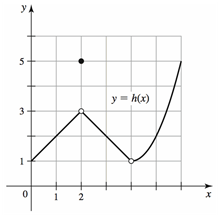
\includegraphics[scale=0.85]{pictures/Ch2Sect2_Exer7}}
\end{column}
\begin{column}{0.50\textwidth}\footnotesize
	Determine the following:

	\vspace{-0.4pc}
	\begin{itemize}\footnotesize
	\item[(a)] $h(1)$
	
	\vspace{-0.25pc}
	\item[(b)] $h(2)$
	
	\vspace{-0.25pc}
	\item[(c)] $h(4)$
	
	\vspace{-0.25pc}
	\item[(d)] $\lim_{x \to 2} h(x)$
	
	
	\vspace{-0.25pc}
	\item[(e)] $\lim_{x \to 4} h(x)$
	
	\vspace{-0.25pc}
	\item[(f)] $\lim_{x \to 1} h(x)$
	\end{itemize}
\end{column}
\end{columns}
\end{exe}
\end{frame}

% % %
\begin{frame}
\begin{que} Does $\lim_{x \to a} f(x)$ always equal $f(a)$? \end{que}
(Hint: Look at the example from the previous slide!)
\end{frame}

% % %
\subsubsection{Determining Limits from a Table}
\begin{frame}{\small Determining Limits from a Table}
\begin{exe} Suppose $f(x)=\dfrac{x^2+x-20}{x-4}$.

\begin{itemize}
\item[(a)] Create a table of values of $f(x)$ when
\begin{alignat*}{3}
x &= 3.9, 3.99, 3.999,\ \text{and}\\
x &= 4.1, 4.01, 4.001
\end{alignat*}
\item[(b)] What can you conjecture about $\lim_{x \to 4} f(x)$?
\end{itemize}
\end{exe}
\end{frame}

% % %
\subsubsection{One-Sided Limits}
\begin{frame}{\small One-Sided Limits}
Up to this point we have been working with two-sided limits; however, for some functions it makes sense to examine one-sided limits.  

\vspace{2pc}
Notice how in the previous example we could approach $f(x)$ from both sides as $x$ approaches $a$, i.e., when $x>a$ and when $x<a$.  
\end{frame} 

% % %
\begin{frame}\footnotesize
\begin{dfn}[right-hand limit] Suppose $f$ is defined for all $x$ near $a$ with $x>a$.  If $f(x)$ is arbitrarily close to $L$ for all $x$ sufficiently close to $a$ with $x>a$, we write

\vspace{-0.5pc}
\[\lim_{x \to a^+} f(x)=L\]

\vspace{-0.25pc}
and say {\bf the limit of $f(x)$ as $x$ approaches $a$ from the right equals $L$}. \end{dfn}

\begin{dfn}[left-hand limit] Suppose $f$ is defined for all $x$ near $a$ with $x<a$.  If $f(x)$ is arbitrarily close to $L$ for all $x$ sufficiently close to $a$ with $x<a$, we write

\vspace{-0.5pc}
\[\lim_{x \to a^-} f(x)=L\]

\vspace{-0.25pc}
and say {\bf the limit of $f(x)$ as $x$ approaches $a$ from the left equals $L$}. \end{dfn}
\end{frame}

% % %
\begin{frame}
\begin{exe}
\begin{columns}
\begin{column}{.45\textwidth}
	\centering{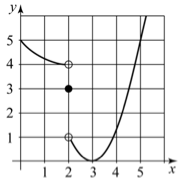
\includegraphics[scale=1]{pictures/Ch2Sect2_QQ7}}
\end{column}
\begin{column}{.45\textwidth}
	Determine the following:
	
	\vspace{0.25pc}
	\begin{itemize}
	\item[(a)] $g(2)$

	\vspace{0.25pc}	
	\item[(b)] $\lim_{x \to 2^+} g(x)$
	
	\vspace{0.25pc}
	\item[(c)] $\lim_{x \to 2^-} g(x)$
	
	\vspace{0.25pc}
	\item[(d)] $\lim_{x \to 2} g(x)$
	\end{itemize}
	\vspace{3pc}
\end{column}
\end{columns}
\end{exe}
\end{frame}

% % %
\subsubsection{Relationship Between One- and Two-Sided Limits}
\begin{frame}{\small Relationship Between One- and Two-Sided Limits}
\begin{thm}\footnotesize If $f$ is defined for all $x$ near $a$ except possibly at $a$, then $\lim_{x \to a} f(x)=L$ if and only if \alert{both} $\lim_{x \to a^+} f(x)=L$ \alert{and} $\lim_{x \to a^-} f(x)=L$. \end{thm}

In other words, the only way for a two-sided limit to exist is if the one-sided limits equal the same number ($L$).
\end{frame}

% % %
\subsubsection{Book Problems}
\begin{frame}
\begin{block}{2.2 Book Problems}1-4, 7, 9, 11, 13, 19, 23, 29, 31 \end{block} 
\end{frame}

% % %
\subsection[2.3 Techniques for Computing Limits]{\S 2.3 Techniques for Computing Limits}
% % %

% % %
\begin{frame}{\S 2.3 Techniques for Computing Limits}\footnotesize
\begin{exe}
Given the function $f(x)=4x+7$, find $\lim_{x\to -2}f(x)$
\begin{enumerate}[(a)]
	\item graphically;
	\item numerically (i.e., using a table of values near $-2$)
	\item via a direct computation method of your choosing.
	\end{enumerate}
\end{exe}

Compare and contrast the methods in this exercise -- which is the most favorable?
\end{frame}

% % %
\begin{frame}{}\footnotesize
This section provides various laws and techniques for determining limits.  These constitute {\bf analytical} methods of finding limits.  The following is an example of a very useful limit law:

\vspace{0.5pc}
{\bf Limits of Linear Functions:}  Let $a$, $b$, and $m$ be real numbers.  For linear functions $f(x)=mx+b$,

\vspace{-0.5pc}
\[\lim_{x \to a} f(x)=f(a)=ma+b.\]

\vspace{0.25pc}
This rule says we if $f(x)$ is a linear function, then in taking the limit as $x\to a$, we can just plug in the $a$ for $x$.

\vspace{0.5pc}
\alert{IMPORTANT!} Using a table or a graph to compute limits, as in the previous sections, can be helpful.  However, ``analytical" does not include those techniques.
\end{frame}

% % %
\subsubsection{Limit Laws}\small
\begin{frame}{\small Limit Laws}{}
{\footnotesize Assume $\lim_{x \to a} f(x)$ and $\lim_{x \to a} g(x)$ exist, $c$ is a real number, and $m,n$ are positive integers.

\hrulefill
}
\begin{itemize}
\item[{\bf 1.}] {\bf Sum:} $\lim_{x \to a}\left(f(x)+g(x)\right) = \lim_{x \to a} f(x)+\lim_{x \to a} g(x)$

\vspace{1pc}
\item[{\bf 2.}] {\bf Difference:} $\lim_{x \to a}\left(f(x)-g(x)\right) = \lim_{x \to a} f(x)-\lim_{x \to a} g(x)$
\end{itemize}

\vspace{0.75pc}
In other words, if we are taking a limit of two things added together or subtracted, then we can first compute each of their individual limits one at a time.
\end{frame}

% % %
\begin{frame}{\small Limit Laws, cont.}{}
{\footnotesize Assume $\lim_{x \to a} f(x)$ and $\lim_{x \to a} g(x)$ exist, $c$ is a real number, and $m,n$ are positive integers.

\hrulefill
}
\begin{itemize}
\item[{\bf 3.}] {\bf Constant Multiple:} $\lim_{x \to a}\left(cf(x)\right) = c\left(\lim_{x \to a}f(x)\right)$

\vspace{1pc}
\item[{\bf 4.}] {\bf Product:}  $\lim_{x \to a}\left(f(x)g(x)\right) = \left(\lim_{x \to a} f(x)\right) \left(\lim_{x \to a} g(x)\right)$
\end{itemize}

\vspace{1.25pc}
The same is true for products.  If one of the factors is a constant, we can just bring it outside the limit.  In fact, a constant is its own limit.
\end{frame}

% % %
\begin{frame}{\small Limit Laws, cont.}{}
{\footnotesize Assume $\lim_{x \to a} f(x)$ and $\lim_{x \to a} g(x)$ exist, $c$ is a real number, and $m,n$ are positive integers.

\hrulefill
}
\begin{itemize}
\item[{\bf 5.}] {\bf Quotient:}  $\lim_{x \to a} \left(\frac{f(x)}{g(x)} \right) = \frac{\displaystyle\lim_{x \to a} f(x)}{\displaystyle\lim_{x \to a} g(x)}$

\vspace{1pc}
(provided $\lim_{x \to a} g(x) \ne 0$)
\end{itemize}

\begin{que}Why the caveat? \end{que}
\end{frame}

% % %
\begin{frame}{\small Limit Laws, cont.}{}\footnotesize
{\footnotesize Assume $\lim_{x \to a} f(x)$ and $\lim_{x \to a} g(x)$ exist, $c$ is a real number, and $m,n$ are positive integers.

\hrulefill
}
\begin{itemize}
\item[{\bf 6.}] {\bf Power:} $\lim_{x \to a}\left(f(x)\right)^n = \left( \lim_{x \to a} f(x) \right)^n$

\vspace{0.4pc}
\item[{\bf 7.}] {\bf Fractional Power:} $\lim_{x \to a} \left(f(x)\right)^{\frac{n}{m}} = \left( \lim_{x \to a} f(x) \right)^{\frac{n}{m}}$ 

\vspace{0.2pc}
(provided $f(x) \ge 0$ for $x$ near $a$ if $m$ is even and $\textstyle\frac{n}{m}$ is in lowest terms)
\end{itemize}

\vspace{-0.3pc}
\begin{que}Explain the caveat in {\bf 7.} \end{que}
\end{frame}

% % %
\begin{frame}{\small Limit Laws, cont.}\footnotesize
Laws {\bf 1.}-{\bf 6.} hold for one-sided limits as well.  But {\bf 7.} must be modified:

\begin{itemize}
\item[{\bf 7.}] {\bf Fractional Power (one-sided limits):} 
	\begin{itemize}
	\item $\lim_{x \to a^{\alert{+}}}\left(f(x)\right)^{\frac{n}{m}} = \left( \lim_{x \to a^{\alert{+}}} f(x) \right)^{\frac{n}{m}}$

	\vspace{0.25pc}
	(provided $f(x) \ge 0$ for $x$ near $a$ \alert{with $x>a$}, if $m$ is even and $\textstyle\frac{n}{m}$ is in lowest terms)
	
	\vspace{0.75pc}
	\item $\lim_{x \to a^{\alert{-}}}\left(f(x)\right)^{\frac{n}{m}} = \left( \lim_{x \to a^{\alert{-}}} f(x) \right)^{\frac{n}{m}}$ 
	
	\vspace{0.25pc}
	(provided $f(x) \ge 0$ for $x$ near $a$ \alert{with $x<a$}, if $m$ is even and $\textstyle\frac{n}{m}$ is in lowest terms)
	\end{itemize}
\end{itemize}
\end{frame}

% % %
\subsubsection{Limits of Polynomials and Rational Functions}
\begin{frame}{\small Limits of Polynomials and Rational Functions}{}\footnotesize
Assume that $p(x)$ and $q(x)$ are polynomials and $a$ is a real number.

\vspace{0.6pc}
\begin{itemize}
\item {\bf Polynomials:}  $\lim_{x \to a} p(x) = p(a)$

\vspace{0.4pc}
\item {\bf Rational functions:}  $\lim_{x \to a} \frac{p(x)}{q(x)} = \frac{p(a)}{q(a)}$ 

\vspace{0.1pc}
(provided $q(a) \ne 0$)
\end{itemize}

\vspace{0.6pc} 
For polynomials and rational functions we can plug in $a$ to compute the limit, as long as we don't get zero in the denominator.  Linear functions count as polynomials.  A rational function is a ``fraction" made of polynomials.
\end{frame}

% % %
\begin{frame}\footnotesize
\begin{exe} Evaluate the following limits analytically.
\begin{itemize}
\item[1.\quad] $\lim_{x \to 1}\frac{4f(x)g(x)}{h(x)}$, given that 

\vspace{-0.25pc}
\[\lim_{x \to 1} f(x)=5, \; \lim_{x \to 1} g(x)=-2, \;\text{and }\lim_{x \to 1} h(x)=-4.\]

\vspace{0.1pc}
\item[2.\quad] $\lim_{x \to 3} \frac{4x^2+3x-6}{2x-3}$

\vspace{0.5pc}
\item[3.\quad] $\lim_{x \to 1^-}g(x)$ \;and\; $\lim_{x \to 1^+}g(x)$, given that

\vspace{-0.25pc}
\[g(x) = 
\begin{cases}
x^2 & \text{if $x \le 1$}; \\
x+2 & \text{if $x>1$}.
\end{cases}
\] 
\end{itemize}
\end{exe}
\end{frame}

\end{document}